\documentclass[9pt,landscape]{article}
\usepackage{{./../static/style}}
\pdfinfo{
  /Title (PyAnsys Cheat Sheet)
  /Creator (TeX)
  /Producer (pdfTeX 1.40.0)
  /Author (Ansys)
  /Subject (PyAnsys)
  /Keywords (PyAnsys, Cheat sheet, template)}

\begin{document}
\raggedright
\footnotesize

% Add the title of cheat sheet here
% ----------------------------------------
\begin{center}
     \Huge{\textbf{PyFluent Cheat sheet}} \\
\end{center}
\begin{center}
     \Large{\textbf{Solver Settings Object Interface}} \\
     \small{\textbf{version:0.13 (stable)}} \\
\end{center}

\AddToShipoutPicture*
  {\put(670,577.5){
\includegraphics[height = 1.2cm]{ansys.png}}}
\AddToShipoutPictureBG*{
\includegraphics[width=\paperwidth]{bground.png}}
\vspace{-0.15cm}
\noindent\makebox[\linewidth]{\rule{\paperwidth}{2pt}}

\begin{multicols}{3}
\setlength{\premulticols}{1pt}
\setlength{\postmulticols}{1pt}
\setlength{\multicolsep}{1pt}
\setlength{\columnsep}{2pt}

% session starts here. 
% First colomn
% --------------------------------------------------------------------------------
\vfill
\section{
\includegraphics[height=\fontcharht\font`\S]{slash.png} Launch Fluent locally}

\pythoncode{scripts/generated_scripts/pyfluent_script_1.py}

% row 2 col 1
\section{
\includegraphics[height=\fontcharht\font`\S]{slash.png} Import mesh in launched session}

The following examples show how to read the available mesh file in Fluent Session.

\pythoncode{scripts/generated_scripts/pyfluent_script_2.py}

There are other specific methods available for reading case files and
reading case-data files. 

\pythoncode{scripts/generated_scripts/pyfluent_script_3.py}


% row 3 col 1
\section{
\includegraphics[height=\fontcharht\font`\S]{slash.png} Enable heat transfer physics}

The following examples show how to enable heat transfer by activating the energy equation.

\pythoncode{scripts/generated_scripts/pyfluent_script_4.py}

\section{
\includegraphics[height=\fontcharht\font`\S]{slash.png} Accessing the \textbf{object state} with using \textbf{pprint}}

\pythoncode{scripts/generated_scripts/pyfluent_script_5.py}


% Second column
% --------------------------------------------------------------------------------
% row 1 col 2
\vfill
\section{
\includegraphics[height=\fontcharht\font`\S]{slash.png}  Define materials}
This example shows how you use Solver settings objects to define materials.
\pythoncode{scripts/generated_scripts/pyfluent_script_6.py}

% row 2 col 2
\section{
\includegraphics[height=\fontcharht\font`\S]{slash.png}  Define boundary conditions}

The examples in this section show how you use Solver settings objects to define boundary conditions.
\pythoncode{scripts/generated_scripts/pyfluent_script_7.py}

\vfill
\section{{
\includegraphics[height=\fontcharht\font`\S]{slash.png}  Modify \textbf{cell zone} conditions}} \\
The examples in this section show how you use Solver settings objects to modify \textbf{cell zone} conditions.
\pythoncode{scripts/generated_scripts/pyfluent_script_8.py}
\vfill

% Third column
% --------------------------------------------------------------------------------
\vfill
% row 1 col 3
\section{
\includegraphics[height=\fontcharht\font`\S]{slash.png}  Apply solution settings}
PyFluent allows you to use Solver settings objects to apply
solution settings, initialize, and solve.

\pythoncode{scripts/generated_scripts/pyfluent_script_9.py}

% row 2 col 3
\section{
\includegraphics[height=\fontcharht\font`\S]{slash.png}  Post-Processing}
PyFluent allows you to post-process data with \textbf{results} object. The following example shows you how to create and display contours on a plane.

\pythoncode{scripts/generated_scripts/pyfluent_script_10.py}
\section{
\includegraphics[height=\fontcharht\font`\S]{slash.png}  Temperature Contour}
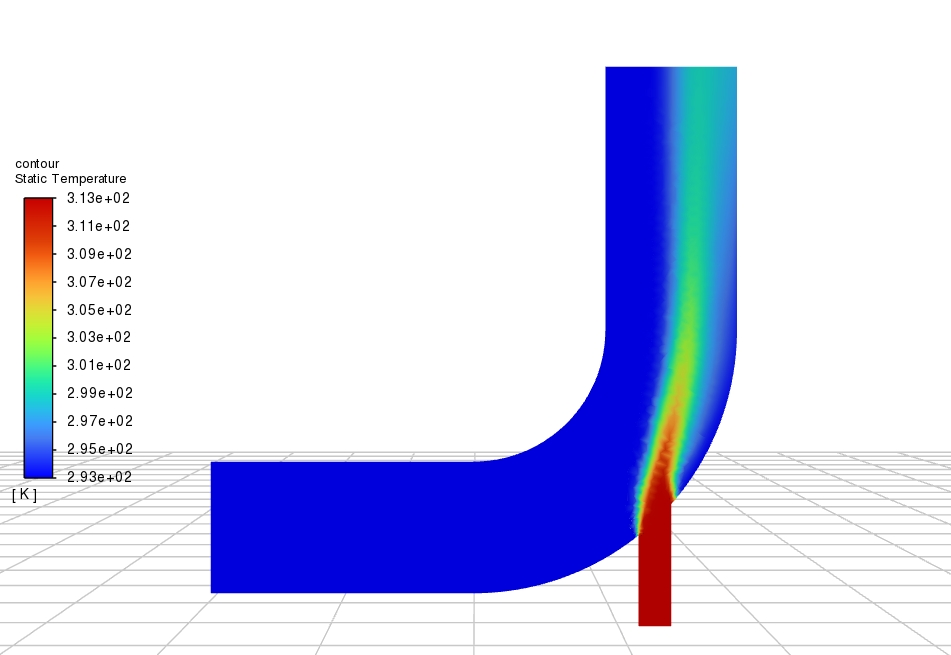
\includegraphics[scale=0.15]{mixing_elbow_pyfluent.jpg}
\centering


% Add subsection
% This section includes useful links to the documentation.
% Examples: installation, API reference, commands, examples.
% Replace 'name of link' with appropriate display text.

\subsection{References from PyFluent Documentation}
\begin{itemize}
\item \href{https://fluent.docs.pyansys.com/version/stable/getting_started/index.html}{\color{blue}{Getting Started}}  
\item \href{https://fluent.docs.pyansys.com/version/stable/api/solver/settings.html#ref-settings}{\color{blue}{PyFluent Solver Settings Objects}}
\item \href{https://fluent.docs.pyansys.com/version/stable/examples/index.html}{\color{blue}{PyFluent Examples}}
\end{itemize}
\end{multicols}

% Footer session of the latex with link to documentation and GitHub page
\vspace{-0.15cm}
\noindent\makebox[\linewidth]{\rule{\paperwidth}{4pt}}
\begin{center}
Getting Started with PyFluent 
\includegraphics[height=\fontcharht\font`\S]{slash.png} \href{https://github.com/ansys/pyfluent}{\color{blue}{PyFluent on GitHub}}} 
\includegraphics[height=\fontcharht\font`\S]{slash.png} Visit \code{\href{https://fluent.docs.pyansys.com/}}{\color{blue}{fluent.docs.pyansys.com}}
\end{center}
\end{document}
